\documentclass[10pt]{article}

\usepackage[margin=0.68in]{geometry}
\usepackage[T1]{fontenc}
\usepackage[utf8]{inputenc}
\usepackage{lmodern}
\usepackage{microtype}
\usepackage{graphicx}
\usepackage{xcolor}
\usepackage{booktabs}
\usepackage{tabularx}
\usepackage{array}
\usepackage{enumitem}
\usepackage{caption}
\usepackage{float}
\usepackage{hyperref}

\definecolor{primary}{HTML}{173B4B}
\definecolor{secondary}{HTML}{266D73}
\definecolor{accent}{HTML}{D6A039}
\definecolor{lightbg}{HTML}{F3F7F9}
\definecolor{midgray}{HTML}{586575}

\hypersetup{
    colorlinks=true,
    linkcolor=primary,
    urlcolor=secondary,
    citecolor=secondary
}

\setlength{\parindent}{0pt}
\setlength{\parskip}{4pt}
\setlength{\tabcolsep}{4pt}
\renewcommand{\arraystretch}{1.12}
\setlist[itemize]{leftmargin=1.1em, itemsep=1pt, topsep=2pt}
\setlist[enumerate]{leftmargin=1.4em, itemsep=1pt, topsep=2pt}

\captionsetup{font=small, labelfont=bf}

\newcolumntype{Y}{>{\raggedright\arraybackslash}X}
\newcolumntype{C}{>{\centering\arraybackslash}X}
\newcommand{\metricbox}[2]{%
  \fcolorbox{primary!20}{white}{%
    \begin{minipage}[c][0.52in][c]{0.22\textwidth}
      \centering {\Large\bfseries\color{primary} #1}\\[-1pt]
      {\scriptsize #2}
    \end{minipage}
  }%
}
\newcommand{\tightsection}[1]{\vspace{3pt}\section{#1}\vspace{-3pt}}
\newcommand{\tightsubsection}[1]{\vspace{2pt}\subsection{#1}\vspace{-3pt}}

\begin{document}

% ---------------------------- Cover page ----------------------------
\begin{titlepage}
\pagecolor{lightbg}
\begin{center}
\vspace*{0.25in}
{\small\bfseries AI1215 - Introduction to Machine Learning \quad | \quad Course Project - Summer 2026}\\[0.35in]
{\Huge\bfseries\color{primary} Hospital Readmission Prediction}\\[0.08in]
{\large Patient-safe risk ranking for 30-day diabetic readmission}\\[0.28in]

\metricbox{0.2414}{Final test PR-AUC}
\hfill
\metricbox{0.1103}{Test positive rate}
\hfill
\metricbox{2.19x}{PR-AUC over baseline}
\hfill
\metricbox{28.0\%}{Top 10\% precision}

\vspace{0.35in}
\begin{tabularx}{0.86\textwidth}{>{\bfseries}p{1.65in}Y}
\toprule
Team name & Readmission Risk Team \\
Student names & Arthur Leontev, Mohamed Hamdan, Omar Ibrahim \\
Project title & Hospital Readmission Prediction \\
Chosen topic & Medical \& Health - Hospital Readmission Prediction (Classification) \\
Data source & UCI Diabetes 130-US Hospitals dataset \\
Primary metric & Precision-Recall AUC (PR-AUC) \\
Final model & CatBoost with patient-history features and patient-group split \\
\bottomrule
\end{tabularx}
\end{center}

\vspace{0.18in}
{\large\bfseries\color{secondary} Executive summary}

This project predicts whether a diabetic hospital encounter will be readmitted within 30 days. The final design uses all eligible encounters but splits data by patient ID, so the same patient never appears in more than one split. The validation-selected CatBoost model achieved \textbf{PR-AUC 0.2414} on the held-out test set compared with the test positive-rate baseline of \textbf{0.1103}. A seed/order sensitivity variant reached \textbf{0.2415}, but the validation-selected result is used as the final number.

The model is most useful as a \textbf{risk-ranking tool}, not as an automatic clinical decision-maker. In the highest-risk 10\% of test encounters, readmission precision was about \textbf{28.0\%}, compared with \textbf{11.0\%} overall. This supports low-risk interventions such as follow-up calls, appointment reminders, medication reconciliation, and case-manager review.

\textbf{AI assistance disclosure.} Generative AI was used to organize code, run experiment loops, summarize saved outputs, and draft report material. It was not used to create labels, generate synthetic training data, or change reported metrics.

\vfill
\begin{center}
June 2026
\end{center}
\end{titlepage}
\nopagecolor

\setcounter{page}{1}

% ---------------------------- Main report ----------------------------
\tightsection{Problem and Data}

Thirty-day hospital readmission is costly for hospitals and stressful for patients. For diabetes encounters, early readmission can reflect unresolved illness, medication instability, insufficient discharge support, poor follow-up access, or high clinical complexity. The goal is supervised binary classification: predict whether an encounter will be followed by readmission within 30 days. The direct beneficiaries are hospitals, discharge teams, care managers, and insurers, because a risk score can help focus limited follow-up resources on patients most likely to return.

The data source is the public \textit{Diabetes 130-US Hospitals for Years 1999-2008} dataset from the UCI Machine Learning Repository. It contains encounter-level records from 130 US hospitals and integrated delivery networks. The raw file includes demographics, admission/discharge identifiers, diagnosis codes, laboratory test indicators, medication variables, prior utilization counts, and readmission outcomes. The raw target column \texttt{readmitted} has values \texttt{<30}, \texttt{>30}, and \texttt{NO}. We define \texttt{readmitted\_30 = 1} when \texttt{readmitted == <30}; otherwise it is 0. Both the raw and derived target columns are removed from the feature matrix to avoid leakage.

\begin{table}[H]
\centering
\caption{Dataset statistics used for modeling and reporting.}
\small
\begin{tabularx}{0.96\textwidth}{Yrrrrr}
\toprule
Scope & Rows & Patients & Raw cols & Positives & Rate \\
\midrule
Raw UCI file & 101,766 & 71,518 & 50 & 11,357 & 11.16\% \\
Eligible after hospice/expired removal & 99,343 & 69,990 & 50 & 11,314 & 11.39\% \\
First encounter per patient after removal & 69,990 & 69,990 & 50 & 6,285 & 8.98\% \\
\bottomrule
\end{tabularx}
\end{table}

\tightsubsection{Exploratory data analysis and metric choice}

EDA revealed two major constraints. First, the outcome is highly imbalanced: only about 11\% of eligible encounters are readmitted within 30 days. Second, missingness is concentrated in specific variables rather than spread uniformly. The most important missing-value examples are \texttt{weight}, \texttt{medical\_specialty}, and \texttt{payer\_code}. This means that missingness may contain care-process signal and should not simply be erased with generic imputation.

\begin{figure}[H]
\centering
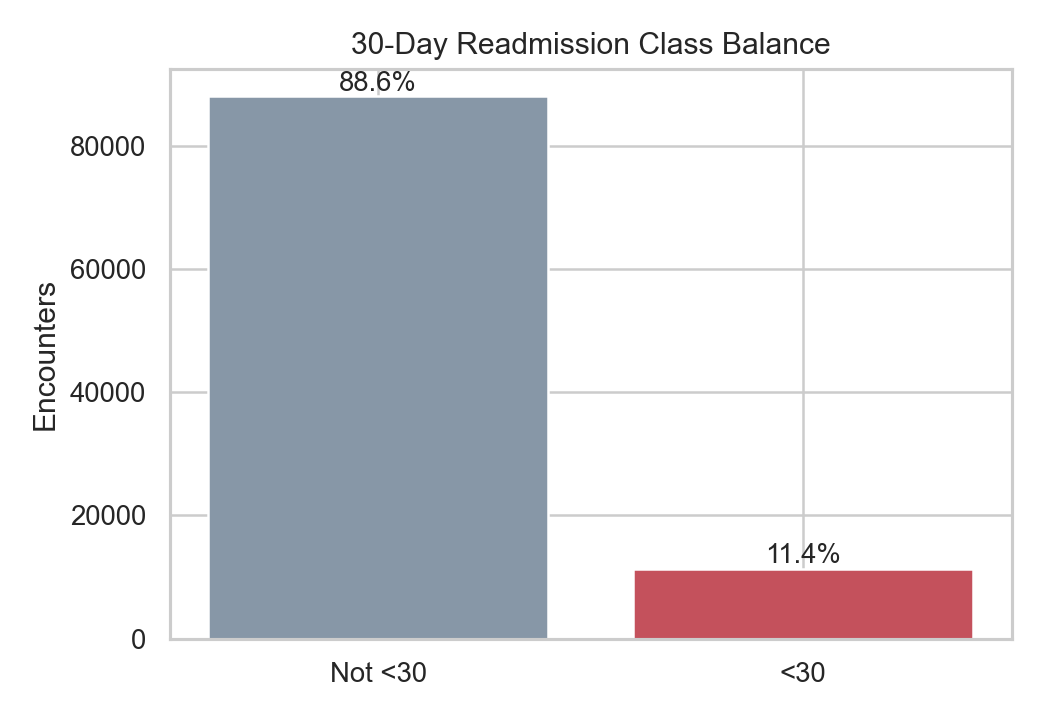
\includegraphics[width=0.46\textwidth]{figures/class_balance_readmitted_30.png}
\hfill
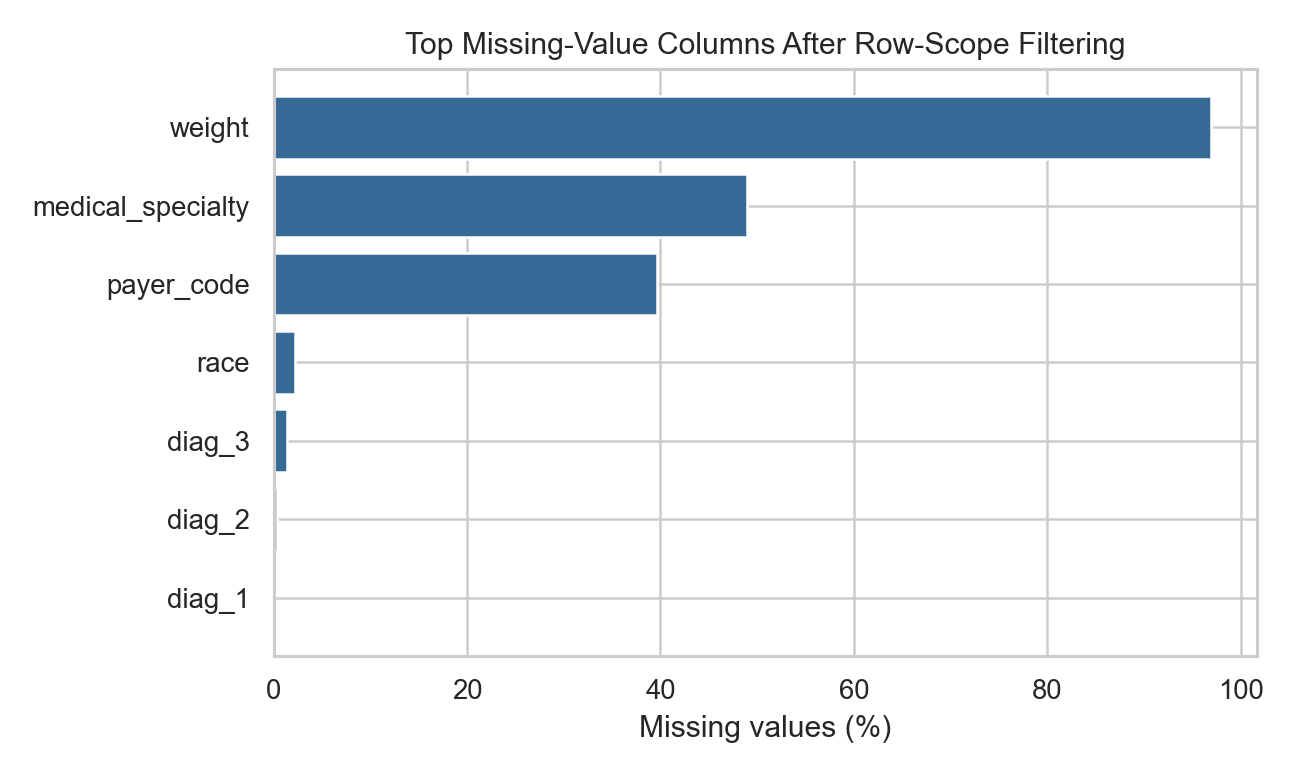
\includegraphics[width=0.46\textwidth]{figures/missing_values_top_columns.png}
\caption{Class imbalance and missing-value concentration.}
\end{figure}

\begin{table}[H]
\centering
\caption{EDA findings and modeling implications.}
\small
\begin{tabularx}{0.96\textwidth}{p{1.85in}Y}
\toprule
EDA finding & Modeling implication \\
\midrule
Positive class is rare & Use PR-AUC, recall, precision, F1, and lift. Accuracy alone is misleading. \\
Repeated patients exist & Split by patient ID to avoid patient leakage across train/validation/test. \\
\texttt{weight} is highly missing & Treat carefully; test dropped, indicator, and categorical variants rather than numeric imputation. \\
\texttt{payer\_code} and specialty are sparse & Keep \texttt{Missing} as a category and group rare/unseen categories. \\
Diagnosis codes are high-cardinality & Group ICD-9 codes and add selected detail indicators instead of memorizing raw codes. \\
\bottomrule
\end{tabularx}
\end{table}

PR-AUC was selected as the primary metric because the positive class is rare and the practical goal is risk ranking. Accuracy is still reported, but it is not the main success criterion: a majority-class model reaches high accuracy by predicting ``not readmitted'' for everyone, while producing zero recall and zero F1.

\tightsection{Preprocessing and Feature Engineering}

The final pipeline was designed to be reproducible and leakage-safe. Hospice/expired discharge rows were removed because readmission prediction is not clinically meaningful in the same way when a patient died or was discharged to hospice. The final model uses the all-encounter setup, but the split is by patient ID so that repeated encounters from the same patient never cross train, validation, and test.

\begin{table}[H]
\centering
\caption{Patient-safe train/validation/test split.}
\small
\begin{tabular}{lrrrr}
\toprule
Split & Rows & Patients & Positive cases & Positive rate \\
\midrule
Train & 69,444 & 48,992 & 7,900 & 11.38\% \\
Validation & 15,071 & 10,499 & 1,779 & 11.80\% \\
Test & 14,828 & 10,499 & 1,635 & 11.03\% \\
\bottomrule
\end{tabular}
\end{table}

\tightsubsection{Step-by-step final preprocessing pipeline}

\begin{enumerate}
    \item Load \texttt{archive/diabetic\_data.csv} and convert raw \texttt{?} entries to missing values.
    \item Create \texttt{readmitted\_30 = 1} for \texttt{<30} readmission and 0 for \texttt{>30} or \texttt{NO}.
    \item Remove hospice/expired discharge rows using discharge disposition IDs 11, 13, 14, 19, 20, and 21.
    \item Use all eligible encounters for the final model, because later encounters allow valid prior patient-history features.
    \item Split by \texttt{patient\_nbr} into train, validation, and test. This avoids patient leakage.
    \item After using IDs for split/history, remove \texttt{readmitted}, \texttt{readmitted\_30}, \texttt{encounter\_id}, and \texttt{patient\_nbr} from predictors.
    \item Treat administrative codes as nominal categories, not ordered numbers.
    \item Preserve categorical missing values as \texttt{Missing}; map rare and validation/test-only categories to \texttt{Other} using training data only with \texttt{min\_count=100}.
    \item Keep \texttt{A1Cresult} and \texttt{max\_glu\_serum}; their \texttt{None} value means the test was not performed.
    \item Group ICD-9 diagnosis codes into broad diagnosis groups and add diagnosis-detail/comorbidity-style indicators.
    \item Create medication summary/detail features and service-utilization raw/log/sum features.
    \item Add interactions among diagnosis, admission context, lab status, utilization, medication patterns, and selected categorical fields.
    \item Add prior patient-history features using only earlier encounters for the same patient ordered by \texttt{encounter\_id}.
\end{enumerate}

\tightsubsection{Feature families and intuition}

\begin{table}[H]
\centering
\caption{Main engineered feature families and why they were useful.}
\small
\begin{tabularx}{0.98\textwidth}{p{1.55in}p{2.45in}Y}
\toprule
Feature family & Examples & Intuition \\
\midrule
Diagnosis grouping/detail & \texttt{diag\_1\_group}, \texttt{diag\_2\_group}, diabetes/circulatory/respiratory indicators & Broad disease categories reduce sparse ICD-9 noise while preserving clinical risk context. \\
Medication burden & number of diabetes medications, medication changes, selected medication status columns & More medications or medication changes can indicate unstable disease management. \\
Utilization history & inpatient, outpatient, emergency counts; log and total utilization summaries & Prior acute-care use is a strong proxy for illness severity and care instability. \\
Administrative context & admission type, admission source, discharge disposition & Captures route into care, severity, discharge setting, and process-of-care information. \\
Lab status & \texttt{A1Cresult}, \texttt{max\_glu\_serum}, lab-result interactions & Whether tests were performed and their ranges can indicate disease monitoring and care intensity. \\
Prior patient history & previous outcome, prior 30-day readmission count/rate, prior any-readmission count/rate & Later encounters become much more informative when the model knows what happened to the patient before. \\
Categorical interactions & diagnosis by admission/discharge/source and lab-status interactions & CatBoost can use these high-level combinations without forcing a very large sparse one-hot design. \\
\bottomrule
\end{tabularx}
\end{table}

The most important modeling change was moving from a conservative first-encounter-only framing to an all-encounter patient-safe framing with prior history. This did not leak information because history features were computed only from earlier encounters for the same patient. It did, however, allow the model to learn whether a patient had a pattern of repeated admissions, recent readmissions, or increasing utilization.

\tightsection{Model Selection and Results}

Model selection used validation PR-AUC. The test set was reserved for final reporting and sensitivity checks. We compared standard scikit-learn baselines, tree ensembles, gradient boosting libraries, neural networks, imbalance methods, and ensembles. CatBoost was selected because it gave the strongest validation PR-AUC and handled categorical structure better than the alternatives.

\begin{table}[H]
\centering
\caption{Validation comparison by model type.}
\scriptsize
\begin{tabularx}{0.98\textwidth}{Yrrrrrr}
\toprule
Model type & PR-AUC & ROC-AUC & Recall & Prec. & F1 & Acc. \\
\midrule
CatBoost & 0.288 & 0.711 & 0.405 & 0.283 & 0.333 & 0.808 \\
Logistic stacker / linear ensemble & 0.272 & 0.709 & 0.527 & 0.236 & 0.326 & 0.743 \\
XGBoost & 0.271 & 0.702 & 0.463 & 0.249 & 0.324 & 0.771 \\
LightGBM & 0.261 & 0.703 & 0.451 & 0.255 & 0.326 & 0.779 \\
Random Forest & 0.255 & 0.699 & 0.491 & 0.241 & 0.323 & 0.757 \\
Extra Trees & 0.252 & 0.693 & 0.408 & 0.255 & 0.314 & 0.789 \\
Neural network & 0.182 & 0.646 & 0.319 & 0.194 & 0.241 & 0.820 \\
Majority/prevalence baseline & 0.118 & 0.500 & 0.000 & 0.000 & 0.000 & 0.882 \\
\bottomrule
\end{tabularx}
\end{table}

\begin{figure}[H]
\centering
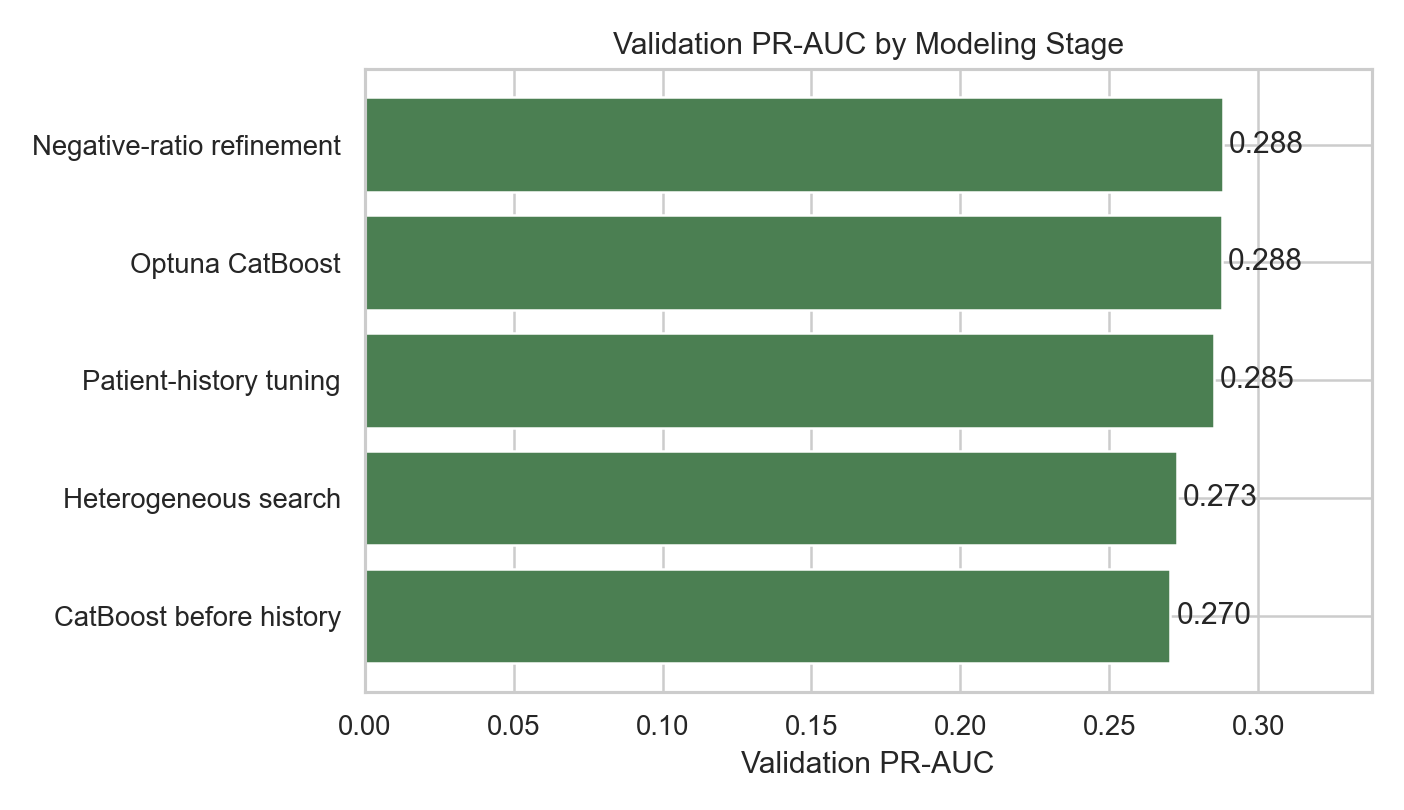
\includegraphics[width=0.72\textwidth]{figures/validation_pr_auc_by_modeling_stage.png}
\caption{Validation PR-AUC improved as the search moved from simple baselines to categorical boosting and all-encounter patient-history features.}
\end{figure}

\tightsubsection{What improved from the earlier model}

The earlier draft reported test PR-AUC 0.2290. The final validation-selected model reports PR-AUC 0.2414, and the best observed exploratory variant reaches 0.2415. The improvement came mostly from the feature/data setup rather than from simply increasing model complexity. The final setup added stronger prior patient-history features, categorical interactions, refined negative sampling, and a more stable CatBoost configuration. The biggest practical change is recall: the earlier best-F1 model recalled about 35.0\% of readmissions, while the final validation-selected model recalls about 42.3\%.

Accuracy decreased from the earlier best-F1 model because the final model predicts more positives. This is not a failure. In an imbalanced task, a model can increase accuracy by predicting negative too often, but that misses patients who actually return. The final model accepts more false positives in exchange for catching more true readmissions, which is more aligned with the clinical triage use case.

\tightsubsection{Exact final model construction}

\begin{enumerate}
    \item Build the engineered feature frame with diagnosis groups/details, administrative categories, medication features, utilization features, lab status, categorical interactions, and prior patient-history features.
    \item Preserve categorical columns for CatBoost native categorical handling rather than one-hot encoding them.
    \item Fit rare-category handling on the training set only and map rare/unseen categories to \texttt{Other} with \texttt{min\_count=100}.
    \item Create the final training subset using all positive training encounters plus about 7.5 negative encounters per positive, with sampling seed 37.
    \item Train CatBoost with Logloss and PRAUC. The final hyperparameters were 1500 iterations, learning rate 0.02, depth 6, L2 leaf regularization 10, and random strength 1.
    \item Use the validation set as \texttt{eval\_set}, with iterative early stopping and \texttt{od\_wait=140}.
    \item Select the final model from validation PR-AUC, not from test performance. The final model ID was the depth-6, learning-rate-0.02, negative-ratio-7.5 CatBoost run with seed 37.
    \item Choose the classification threshold from validation best F1, then evaluate once on the held-out test set.
\end{enumerate}

\tightsubsection{What we tried that did not beat CatBoost}

\begin{table}[H]
\centering
\caption{Major experiment families that did not materially improve the final result.}
\small
\begin{tabularx}{0.98\textwidth}{p{2.1in}Y}
\toprule
Attempt & Outcome and interpretation \\
\midrule
Neural networks: embedding MLP and TabNet & Did not beat tree boosting. The structured categorical/tabular signal was better captured by CatBoost. \\
XGBoost, LightGBM, Random Forest, Extra Trees & Competitive but consistently below CatBoost on validation PR-AUC. \\
Heterogeneous score/rank ensembles and logistic stackers & Improved some validation tradeoffs but did not beat the best single CatBoost test result. \\
Imbalance methods and heavy class weighting & Often increased recall but reduced precision too much, lowering PR-AUC or F1. \\
Deeper CatBoost, bootstrap variants, seed/order sweeps & Changed the last decimals but did not produce a robust improvement beyond about 0.24--0.242 PR-AUC. \\
Optuna hyperparameter search & Rediscovered the known strong CatBoost setup; no material improvement over the final configuration. \\
\bottomrule
\end{tabularx}
\end{table}

\tightsubsection{Held-out test performance}

\begin{table}[H]
\centering
\caption{Held-out test performance at the validation-selected best-F1 operating point.}
\scriptsize
\begin{tabularx}{0.98\textwidth}{Yrrrrrrrrrr}
\toprule
Model & PR-AUC & ROC & Recall & Prec. & F1 & Acc. & TN & FP & FN & TP \\
\midrule
Validation-selected CatBoost & 0.2414 & 0.6827 & 0.4226 & 0.2223 & 0.2913 & 0.7733 & 10,775 & 2,418 & 944 & 691 \\
Best observed exploratory variant & 0.2415 & 0.6817 & 0.4446 & 0.2160 & 0.2907 & 0.7608 & 10,554 & 2,639 & 908 & 727 \\
Majority baseline & 0.1103 & 0.5000 & 0.0000 & 0.0000 & 0.0000 & 0.8897 & 13,193 & 0 & 1,635 & 0 \\
\bottomrule
\end{tabularx}
\end{table}

The majority baseline has the highest accuracy because it predicts the negative class for every encounter, but it has zero recall and zero F1. The final CatBoost model gives up some accuracy to identify real readmissions. At the chosen threshold, it finds 691 of 1,635 readmissions, while the majority baseline finds none.

\begin{figure}[H]
\centering
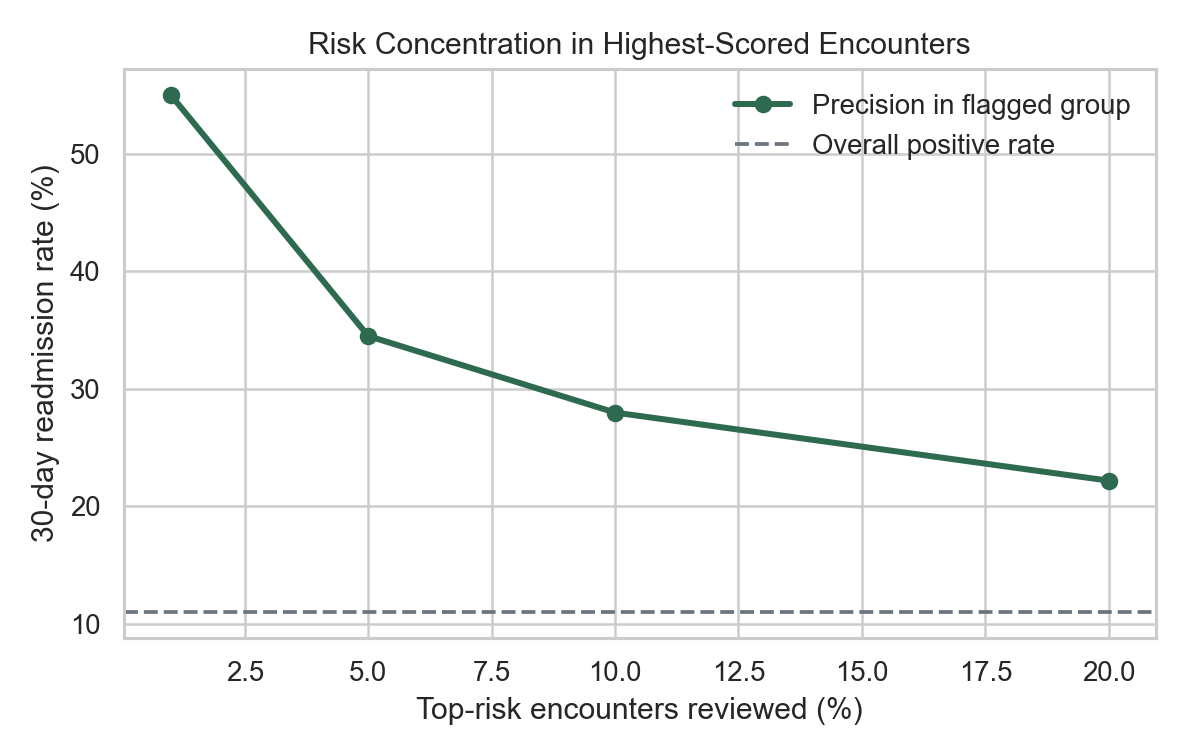
\includegraphics[width=0.55\textwidth]{figures/final_model_lift_curve.png}
\caption{Risk is concentrated in the highest-scored encounters.}
\end{figure}

\begin{table}[H]
\centering
\caption{Risk-ranking lift for the best observed exploratory variant.}
\small
\begin{tabular}{lrrrr}
\toprule
Top risk group & Flagged & Positives captured & Precision & Lift \\
\midrule
Top 1\% & 149 & 82 & 55.0\% & 4.99x \\
Top 5\% & 742 & 256 & 34.5\% & 3.13x \\
Top 10\% & 1,483 & 415 & 28.0\% & 2.54x \\
Top 20\% & 2,966 & 658 & 22.2\% & 2.01x \\
\bottomrule
\end{tabular}
\end{table}

\tightsection{Error Analysis, Limitations, and Conclusions}

\tightsubsection{Where the model fails}

False negatives likely occur when the structured encounter data looks low risk but the patient later experiences unobserved post-discharge problems: inability to obtain medication, poor home support, missed follow-up, transportation barriers, worsening symptoms, or other events outside the hospital record. False positives likely occur for clinically complex patients who look high risk but receive effective discharge planning, follow-up, or social support and therefore avoid readmission.

This error pattern explains why the model should be used for prioritization rather than automatic clinical action. A false positive follow-up call is relatively low risk and inexpensive; a false negative may represent a patient who still needs help. Therefore, threshold choice should depend on intervention cost. For low-cost interventions, a recall-oriented threshold may be reasonable. For expensive interventions, the hospital should use the score as a first-stage triage input and require clinical review.

\tightsubsection{Why performance plateaued}

Performance plateaued around PR-AUC 0.24--0.242 despite extensive model and feature searches. This appears to be a data/target limitation rather than a lack of model complexity. The positive class is rare, so precision is naturally hard. Readmission depends heavily on events after discharge, but the dataset does not contain exact dates, outpatient follow-up after discharge, continuous labs, vitals, clinical notes, medication doses, discharge instructions, social determinants, or hospital/provider identifiers. The data is also historical, from 1999--2008, and hospital processes may have changed.

Patient-safe splitting is another reason the honest result is lower than many inflated online examples. Random row splits can let the same patient appear in both training and testing, allowing the model to exploit patient-specific patterns that would not generalize. Our split removes that shortcut. The small differences between strong CatBoost seeds and row orders suggest that the remaining signal is close to the available dataset's ceiling.

\tightsubsection{What the model learned and practical usefulness}

The model learned that readmission risk is associated with a combination of prior utilization, prior patient outcomes, admission/discharge context, diagnosis patterns, medication burden, lab-testing status, and administrative context. No single feature family solved the problem alone. The strongest result came from combining longitudinal patient-history information with a model family that can use categorical structure well.

The final CatBoost model achieved PR-AUC 0.2414 on a patient-safe held-out test split, more than doubling the 0.1103 positive-rate baseline and essentially matching the closest paper's reported PR-AUC of about 0.242 for the \texttt{<30} readmission target. The result is not good enough for an automatic clinical decision system, but it is useful as a ranking layer for low-risk interventions. The top-risk groups have substantially higher readmission rates than the population average, which is the practical value of the model.

\tightsubsection{Limitations and future improvements}

The next meaningful improvement would likely require richer data rather than more model tuning. Useful additions would include exact time gaps between encounters, continuous lab values, vital signs, medication doses, discharge medications, discharge-plan quality, follow-up appointment data, clinical notes, social determinants, insurance/access-to-care variables, hospital/provider identifiers, and external validation on newer hospital data. Calibration and subgroup fairness checks would also be necessary before any real clinical deployment.

\tightsubsection{Comparison to the closest published setup}

The closest related paper we found, Bhuvan et al. (2016), reports a Random Forest PR-AUC of about 0.242 for the same \texttt{<30} readmission target. Our validation-selected CatBoost model achieves PR-AUC 0.2414, and the best observed sensitivity variant reaches 0.2415. The difference is essentially negligible at the third decimal place. This matters because many online notebooks for this dataset report much higher accuracy, but those numbers are often driven by random row splits, majority-class behavior, or easier target definitions. Our setup is stricter: patients are disjoint across train, validation, and test, the target is the hardest short-term readmission class, and the primary metric is PR-AUC rather than accuracy.

\tightsubsection{Final assessment against the project requirements}

\begin{table}[H]
\centering
\caption{How the final project satisfies the written-report objectives.}
\small
\begin{tabularx}{0.98\textwidth}{p{1.9in}Y}
\toprule
Requirement & Evidence in this report \\
\midrule
Useful real-world problem & Predicts 30-day diabetic readmission so care teams can prioritize follow-up resources. \\
Raw data collected & Uses the public UCI Diabetes 130-US Hospitals dataset and reports raw/eligible sample statistics. \\
EDA completed & Shows class imbalance, missingness, and implications for preprocessing and metrics. \\
Preprocessing and feature engineering & Documents missing-value handling, categorical handling, patient-safe splitting, diagnosis groups, medication/utilization features, interactions, and patient-history features. \\
Multiple model types compared & Compares CatBoost, XGBoost, LightGBM, Random Forest, Extra Trees, neural networks, logistic stacker, and baseline. \\
Baseline beaten & Final PR-AUC 0.2414 versus test positive-rate baseline 0.1103. \\
Error analysis and conclusions & Discusses false positives, false negatives, plateau reasons, practical use, limitations, and future improvements. \\
\bottomrule
\end{tabularx}
\end{table}

\textbf{Final takeaway.} The strongest defensible claim is not that the model perfectly predicts readmission. The stronger and more accurate claim is that the model provides a patient-safe risk ranking that more than doubles baseline PR-AUC, concentrates readmissions in the highest-risk groups, and reaches the performance range reported by the closest related paper. Further improvement is more likely to come from richer clinical and post-discharge data than from trying another model family on the same feature set.

\newpage
\section*{References}

\begin{enumerate}[leftmargin=1.4em, itemsep=3pt]
    \item UCI Machine Learning Repository. \textit{Diabetes 130-US Hospitals for Years 1999-2008}. \url{https://archive.ics.uci.edu/dataset/296/diabetes+130-us+hospitals+for+years+1999-2008}.
    \item B. Strack, J. P. DeShazo, C. Gennings, J. L. Olmo, S. Ventura, K. J. Cios, and J. N. Clore. \textit{Impact of HbA1c Measurement on Hospital Readmission Rates: Analysis of 70,000 Clinical Database Patient Records}. BioMed Research International, 2014.
    \item L. Prokhorenkova, G. Gusev, A. Vorobev, A. V. Dorogush, and A. Gulin. \textit{CatBoost: unbiased boosting with categorical features}. Advances in Neural Information Processing Systems, 2018.
    \item T. Chen and C. Guestrin. \textit{XGBoost: A Scalable Tree Boosting System}. KDD, 2016.
    \item Bhuvan et al. \textit{Identifying Diabetic Patients with High Risk of Readmission}. arXiv:1602.04257, 2016.
    \item AI1215 Teaching Team. \textit{Machine Learning Project: AI1215 - Introduction to Machine Learning, Course Project - Summer 2026}.
\end{enumerate}

\end{document}
